%-------------------------------------------------------------------------------
\chapter{State of the Art}
\labelchapter{ch.state}
%-------------------------------------------------------------------------------

%%%%%%%%%%%%%%%%%%%%%%%%%%%%%%%%%%%%%%%%%%%%%%%%%%%%%%%%%%%%%%%%%%%%%%%%%%%%%%%%
%%%%%%%%%%%%%%%%%%%%%%%%%%%%%%%%%%%%%%%%%%%%%%%%%%%%%%%%%%%%%%%%%%%%%%%%%%%%%%%%

% \vspace{-0.8cm}
\lettrine[lines=2]{T}{his} chapter outlines the related works about \myLongAc{DSE}{Design Space Exploration} on \myLongAc{FPGA}{Field-Programmable Gate Array}.
As the notion of \myAc{DSE} can refer to any process exploring variations of implementations, it can be applied at various levels of granularity, from basic operator implementations \cite{rehman_architectural-space_2016}\cite{geng_high-speed_2021} to whole \myLongAc{SoC}{Systems-on-chip} \cite{ascia_ga-based_2004}\cite{calborean_automatic_2010}, and can even be applied for software/hardware co design \cite{barone_multi-objective_2021}.

Moreover, when it comes to digital design, \myAc{DSE} processes can be applied for both \myLongAc{ASIC}{Application-Specific Integrated Circuit} and \myAc{FPGA} circuits, and some previous works showed that an optimal \myAc{ASIC} solution may prove to be suboptimal when targeting a \myAc{FPGA} \cite{liu2019accelerating}.

In the context of this work, we will hence focus on \myAc{DSE} application at {\bf kernel level}, meaning that we will consider \myAc{FPGA}-based implementations of more or less complex algorithms that fit on a single \myAc{FPGA} device.

We will start by exposing some popular tools leveraging \myAc{DSE} for \myAc{FPGA} based designs, and will consider how are design spaces exposed in the state of the art methodologies.
We will then examine which metrics are used in \myAc{DSE} processes, and how relevant estimators are built and integrated in the exploration frameworks.
Finally, we will discuss various exploration strategies, along with both their advantages and their limitations, before providing a synthesis of the approaches for \myAc{FPGA}-based \myAc{DSE} in the literature.

\clearpage
\vspace*{\fill}
% \clearpage
%Content section
\minitoc 
\vspace*{\fill}
% \mtcskip 
% \minilof

\newpage
%%%%%%%%%%%%%%%%%%%%%%%%%%%%%%%%%%%%%%%%%%%%%%%%%%%%%%%%%%%%%%%%%%%%%%%%%%%%%%%%

\section{Overview of the Existing Tools}
\label{ch.state:seq.tools}

As an exhaustive listing of every \myLongAc{DSE}{Design Space Exploration} framework is both unfeasible and of limited utility, we will start by providing a brief review of the most popular tools aimed at easing the developers life, focusing on rising the abstraction of design processes with approaches such as \myLongAc{HLS}{High Level Synthesis} and \myLongAcs{DSL}{Domain Specific Language}.

To begin with, Windh \etal{} \cite{windh_high-level_2015} provide a rapid study of high level tools for reconfigurable computing.
A particular focus is put on \myAc{HLS} initiatives, with two industrial tools, namely Xilinx Vivado HLS \cite{zhang_autopilot_2008}\cite{xilinx_vivado_2021} and Altera OpenCL \cite{singh2011implementing}, and two academic frameworks, LegUp \cite{canis2011legup} and ROCCC \cite{villarreal_designing_2010}. 
BlueSpec System Verilog \cite{nikhil2008bluespec}, another approach based on a simplified behavioural model --- abstracting some of the difficulties of standard \myLongAcs{HDL}{Hardware Description Language} --- is also introduced.

Whereas the \myAc{HLS} approach is a main trend toward higher productivity, some \myAc{DSL} based initiatives are also considered to close the gap between domain specialists --- such as data scientists or signal processing experts --- on one hand, and \myAc{FPGA} developers on the other.
Kapre \etal{} \cite{kapre_survey_2016} expose a brief survey of different \myAcs{DSL} and their application domains: while DFiant \cite{port_dfiant_2017} focuses on dataflow based applications, Sano \cite{sano_dsl-based_2015} proposes a framework targeting parallel streaming architectures. 
Kristien \etal{} \cite{kristien_high-level_2019} expose how the \texttt{Lift} framework can be used for efficient design, leveraging functional patterns for compilation, while Spatial \cite{koeplinger_spatial_2018} exhibits \myAc{FPGA} specific patterns and constructs for accelerator generation.

All those initiatives demonstrates the variability of the approaches for efficient design, where the abstraction level, the parametrization, the application domain or the target technology are as many knobs that can be tuned to build an efficient design framework.
Most of those approaches rely --- more or less heavily --- on \myAc{DSE} processes to help designers make expertise-based decisions, such as parallelism exhibition, interface definition or dataflow pipelining.

In order to provide an interesting analysis of the existing literature on \myAc{FPGA} based \myAc{DSE}, we thus chose to focus on three main concerns, which we identified as being key levers for efficient strategy definition: 
{\setstretch{0.9}
\begin{itemize}
    \item {\bf design space exposition} --- \ie defining which implementation variations can be explored, and how to generate corresponding architectures
    \item {\bf metric definition} --- \ie exposing metrics of interests for a given use-case, as well as how to build and integrate estimators
    \item {\bf exploration algorithm} --- \ie describing how to scan the design space in a clever way, providing rapid yet accurate results
\end{itemize}
}

\clearpage
\section{Design Space Exposition}
\label{ch.state:sec.space}
    When building a \myAc{DSE} framework, one of the main concerns is to define which variations are to be considered in the exploration, and how to generate the corresponding implementations from the initial description.

    Various abstraction levels are also to be considered, ranging from high level programming languages such as python or C/C++, which can be used to allow software developers to design their own circuits, to \myLongAc{RTL}{Register-Transfer Level} languages, which enable hardware designers to efficiently control the built accelerators based on their expertise.

    However, the input language and the abstraction level can also be considered from another point of view: the level of control over the implementation variations.
    The \myAc{DSE} methodologies can either rely on the explicitation of generation parameters, or on the automatic inference of the implementation variations --- but most of the popular high level tools are based on a mix-up of those two options, allowing users to define some variations while inferring others, based on the standard design methodology (with potential optimizations linked to the application domain and/or the target board).

    In this section, we will hence consider how the design variations are chosen in the different approaches, rather than their abstraction levels.
    Doing so allows to classify the \myAc{DSE} initiatives without introducing the classical distinction between \myAc{HLS}, \myAc{DSL} and other techniques, as the main difference when it comes to exploration is the way to expose the explored design space.

    \subsection{Explicit Parametrization}
    \label{ch.state:sec.space:ssec.explicit}
        
        The basic idea of the explicit parametrization approach is to allow users to define explicit parameters in their code, in order to provide an explorable design space built over understandable variations.
        Such parameters can be application specific, for example matrix dimensions in a matrix multiplication kernel, or independent, with standard parameters such as the \myLongAc{IO}{Input/Output} bandwidth or the element type \cite{ferres_2021_integrating}.

        Application specific generators have been introduced in the literature to easily expose and explore design spaces, at various levels of granularity.
        While Rehman \etal{} \cite{rehman_architectural-space_2016} use a library of basic blocks and the composition of components to explore approximate multiplier implementations, Yiannacouras \etal{} \cite{yiannacouras_exploration_2007} introduce SPREE (Soft Processor Rapid Exploration Environment), a framework allowing to explore the variations of a processor by leveraging standard \myAc{CPU} notions such as \myLongAc{FU}{Functional Unit} implementation and dataflow pipelining.
        Other initiatives have been proposed for domain specific \myAc{DSE}, such as the implementation of \myLongAcs{CNN}{Convolutional Neural Network}, for example using different dataflow techniques as variations \cite{park_roofline-model-based_2020}.
        We can thus state that developers may need to expose very specific parameters in their exploration flow, and the exploration frameworks should provide a way to do so.

        To easily integrate the definition of parameters into the standard design flows, Paletti \etal{} \cite{paletti_dovado_2021} provide {\bf Dovado}, a \myAc{RTL}-based exploration framework leveraging \myAc{HDL} {\it generic} features to build the design space.
        However, their perspectives include supporting other languages with more convenient ways for parametrization, such as \chisel{} or other \myAcs{HCL}.

        \myAcs{HCL} are recent initiatives focused on building parametrizable generators instead of use-case specific accelerators, using high level languages as entry points to leverage promising software paradigms in the hardware world.
        Among them, we can list \python{} based initiatives such as {\bf MyHDL} \cite{jaic2015enhancing} or {\bf PyMTL} \cite{lockhart_pymtl_2014}, \scala{} based frameworks such as \chisel{} \cite{bachrach_chisel_2012} and {\bf SpinalHDL} \cite{papon2017spinalhdl}, and {\bf C$\lambda$ash}, an \haskell{} based project \cite{baaij_clash_2010}.

        Several \chisel{} based initiatives are exploring the possibilities of both high level programming features and highly parametrizable constructors to provide interesting exploration features.
        Cook \etal{} \cite{cook_diplomatic_2017} proposed {\bf Diplomacy}, a parameter negotiation framework to automatically select and propagate generation parameters of the {\bf Rocket chip} processor\footnote{Rocket-chip is an open-source, in-order version of a \chisel{}-based RISC-V processor.} \cite{asanovic_rocket_2016}. 
        To go further, Bai \etal{} introduced the {\bf BOOM-Explorer} \cite{bai_boom-explorer_2021} to explore the \myLongAc{BOOM}{Berkeley Out-of-Order Machine} core\footnote{\myAc{BOOM} is an out-of-order implementation of a \chisel{}-based RISC-V core.}, varying the generation parameters of the different pipeline stages in the dataflow.
        A more generic approach was also provided with {\bf JackHammer} \cite{schmidt_fast_2015}, an exploration framework for \chisel{} based designs.
        However, the initiative is not maintained anymore, and is claimed to be too specific for SHA-3, the target algorithm.

        As one can observe here, exposing explicit parameters through \myAc{HCL} usage seems to be a promising way for an efficient \myAc{DSE} framework definition. 
        Moreover, as \chisel{} is used as a basis for this work, we provide some useful insights and basics in Appendix \ref{app.chisel}, that should help readers to be more familiar with the possibilities that this language offer.

	% \Olivier{Il faut surement dire dans cette section que tous les outils de HLS permettent via des pragmas ou des fichiers de directives de piloter explicitement la génération de l'architecture}
    \subsection{Implicit Inferences}
    \label{ch.state:sec.space:ssec.implicit}

        While a generator-based exploration allows users to define which variations are to be explored, it cannot be used in frameworks based on a change of programming paradigm, such as \myAc{HLS}.
        As \myAc{HLS} is based on translating an algorithmic description to a hardware one, choices are to be taken to model the decisions that a hardware developer would take when doing the same task --- \eg the level of loop unrolling, the memory model or the input bit width.
        While those choices would usually require a lot of parameters and description to be efficient, standard \myAc{HLS} tools often automatically infer which transformations are to be triggered to provide an efficient solution.

        To do so, the \myAc{HLS} flows iteratively select which transforms to perform over the \myLongAc{IR}{Intermediate Representation}, optimizing a certain set of objective functions under constraints \cite{prost-boucle_fast_2014} --- Ye \etal{} \cite{ye_scalehls_2021} even consider a multi-level \myAc{IR} to expose different optimizations depending on the abstraction level.
        Some \myAc{DSL} also use a similar approach for compilation: the {\tt Lift} \cite{kristien_high-level_2019} frameworks expose implementation variations using rewrite rules over the original description, while Sano \etal{} \cite{sano_dsl-based_2015} exploit the inherent parallelism to generate different implementations to be explored.

	% \Olivier{Le calcul approximatif a clairement sa place dans ton état de l'art, mais est-ce vraiment de l'explo implicite dans ces papiers.}
        A similar approach is also used in \myLongAc{AxC}{Approximate Computing} based exploration frameworks, as the actual implementation of used operators does not really matter.
        As a result, different approximations are considered to generate the implementations (named {\it variants} by Witschen \etal{} \cite{witschen_circa_2019}) and build the design space \cite{manuel_model-based_2020}\cite{barone_multi-objective_2021}.
        Other initiatives consider some optimizations that are possible due to the \myAc{AxC} inherent freedom, such as optimizing the data word lengths to reduce required hardware \cite{herve_data_2005} or reordering the floating-point operations to optimize latency \cite{gao_automatically_2016}.

        Those approaches thus bypass both explicit decisions and parameter definition that should be provided by user, and automatically infer how to transform the circuit representation to provide a best fit --- which may result in non optimal designs (with respect to a manually tuned design), and does not allow to fully control generated circuits.

    \subsection{Mixing-up Approaches}
    \label{ch.state:sec.space:ssec.mixing}
        However, when looking to the most popular \myAc{DSE} flows, we can remark that they are actually based on a mix-up of those two approaches.

        To begin with, Schafer \etal{} \cite{schafer_high-level_2020} provide a comprehensive study of the \myAc{HLS} approaches for \myAc{DSE}, and formalize a notion that is key in the design space exposition process: {\bf exploration knobs}.
        Knobs are design parameters exposed at some point in the process, that allow the users to consider the synthesis process as a {\it black box} --- providing different knobs as inputs of the process resulting in a different \myAc{RTL} implementation at the end of it.
        They are classified in three different categories, that are mainly relevant for \myLongAc{ASIC}{Application-Specific Integrated Circuit} design, but can also be considered when targeting a \myAc{FPGA} implementation:

\clearpage

        \begin{itemize}
            \item {\it local synthesis directives}, which are used to control the local inferences of the \myAc{HLS} tool.

                They are often implemented using {\it pragmas} that are directly integrated in the entry code, in order to fix some parameters that would have been inferred by the tool otherwise --- leveraging user expertise.
            \item {\it global synthesis directives}, which are used to specify some global parameters for the synthesis.

                Among them, we can find the scheduling algorithm to be used for compilation, the clock constraints or the \myLongAc{FSM}{Finite State Machine} encoding scheme.
            \item {\it \myAc{FU} constraints}, which defines the level of sharing of \myAcs{FU}, introducing a performance/area trade-off.

                Such knob is often not considered by \myAc{FPGA} targeting \myAc{HLS} tools, as sharing a \myAc{FU} on \myAc{FPGA} often requires more resources (mainly muxes) than implementing another computation unit.% \cite{schafer_high-level_2020}.
        \end{itemize}

        The popular \myAc{HLS} tools mainly leverage {\it local synthesis directives}, as it allows to finely control generated hardware.
        However, defining such {\it pragmas} is often a tedious task, as their impact on the generated circuit is often difficult to understand and may vary depending on the compiler version, which requires an expertise about both hardware development and used \myAc{HLS} flow.
        Moreover, it is difficult to modify the base code, as reusing the behavioural description in another context will probably require to tune every {\it pragmas} again, to guide the exploration flow.

        Another approach based on controllable yet automatic inferences as been introduced in {\bf Spatial} \cite{koeplinger_spatial_2018}, where automatic inferences for scheduling and pipelining coexist with user defined parameters for generation.

    \subsection{Exposing an Explorable Design Space}

        We remark that exposing an interesting design space to be explored --- \ie a design space that consider potentially optimal designs for the current use case while providing a structure enabling an efficient exploration --- often requires the developers to bring their expertise using custom parameters, while some freedom can be left to the tool for simple optimizations in order to allow compact but usable descriptions.

        In this way, we consider building an \myLongAc{HCF}{Hardware Construction Framework} based approach for \myAc{DSE}, to allow users to expose specific parameters for the exploration, while allowing automatic transforms --- which should be easily configurable --- to be performed before generation.

\clearpage
\section{Metric Definition and Estimations}
\label{ch.state:sec.metric}
    Another important concern when it comes to \myAc{DSE} is how to define the {\bf goal} of the exploration.
    As stated by Schafer \etal{} \cite{schafer_high-level_2020}, no generic exploration strategy can be defined as it depends on a lot of parameters such as the application specificities, the target, the functioning conditions or the use-case constraints and objectives.
    An exploration process is thus to be defined specifically for a given combination of those parameters, including the objective function(s) to be optimized through the flow --- as a matter of fact, multiple objectives and/or constraints are often to be considered in such processes to provide usable solutions.
    Barone \etal{} \cite{barone_multi-objective_2021} introduce the need for efficient \myLongAc{MOP}{Multi-objective Optimization Problem} solving --- \ie "finding, for some {\it decision variables}, a set of values satisfying {\it imposed constraints}, while optimizing a set of {\it objective functions}" \cite{osyczka1985multicriteria}.

    In this context, we hence aim at providing some insights about interesting metrics and corresponding estimation methodologies for \myAc{DSE}: in other terms, we want to discuss how two implementations can be compared for a given set of constraint(s) and objective(s).
    Two complementary notions will be considered in this section: {\bf metric definition}, which corresponds to circuit properties that hardware developers consider when iterating over their designs, and {\bf estimation methodologies}, which are the ways those metrics are estimated in the flow.

    Actually, to be able to efficiently explore a design space, an {\bf accuracy} {\it vs} {\bf speed} trade-off is introduced in the process, as providing an accurate estimation of a metric may require long procedures from specific tools --- \eg vendor frameworks such as \vivado{} or \quartus{} --- while quick estimation methodologies often result in approximate estimations.
    We will thus consider mainstream metrics for exploration process, as well as interesting methodologies for their estimations, in order to provide users with a way to comprehend and take the best of this trade-off in their \myAc{DSE} design.
    % \needed{Small intro about how to define the metrics, which are commons, which are usefull}
    
    \subsection{Estimating Temporal and Spatial Concerns}
    \label{ch.state:sec.metric:ssec.resource}
        In standard \myAc{FPGA} processes, developers mainly consider two concerns for validating a circuit --- that it fits the target board, and that the temporal behaviour respects the performance constraints.

        The temporal behaviour is mainly considered using {\bf two metrics}: {\bf functioning frequency}, which defines the clock cycle duration for the design, and {\bf latency}, which is an abstract notion considering the number of cycles needed for a computation (\eg{} in stream based applications such as \myLongAc{FIR Filter}{Finite Impulse Response Filter}, it can be defined as the number of cycles needed for an input sample to have an impact on the kernel output).
        It can also be defined by combining those two metrics, providing a global latency metric in second.

        On the other hand, the spatial part is mainly divided in {\bf four metrics} for \myAc{FPGA} design, corresponding to the basic elements of a \myAc{FPGA} structure:
        \begin{itemize}
            \item \myLongAcs{LUT}{Look-Up Table}%, which are the basic blocks for logic operation implementation
            \item \myLongAcs{FF}{Flip Flop}%, which are basic memory elements used for register implementation
            \item \myLongAcs{DSP}{Digital Signal Processor}%, which are dedicated \myAcs{FU} for specific operations such as multiplication
            \item embedded memories, such as \myLongAcs{BRAM}{Block RAM}%, which are wider memory elements
        \end{itemize}

        Estimations for both metrics are classically based on manual analysis of vendor synthesis or implementation reports, which can hence be used as the {\bf reference value} to achieve through estimations, but is obtained after long processes.
        We will hence discuss different levels of estimations, from high abstraction level to \myAc{RTL} based methodology, to provide insights about speed, accuracy and usability of different methodologies.

        \subsubsection{Resource Estimation} 
            To begin with, resource estimation is a key feature for efficient exploration, with various level approaches proposed the last decades.

            As \myAc{RTL} approaches are easy to integrate in any design flow (the representation level being the entry point of most synthesis flows), \myAc{HDL} based methodologies have been proposed for resource estimation.
            They mainly rely on two complementary approaches: modelling steps that the synthesis is expected to take in order to provide realistic estimations \cite{schumacher_fast_2008}, and use characterisation of basic blocks and \myLongAc{IP}{Intellectual Property} cores \cite{deng_accurate_2008}.
            This characterization approach allows to adapt estimators to a given \myAc{FPGA} and synthesis flow by providing a target specific way to generate the basis of the estimation methodology --- to do so, basic blocks of interests are identified and synthesized only once, the report being parsed to provide a characterized model of the component to be used each time a similar component is identified in the estimated circuit.

            As for higher abstraction initiatives, {\bf MATLAB} based approaches have been introduced for early estimation of resource from algorithmic description through analytical models of circuits \cite{nayak_accurate_2002}\cite{hutchison_system_2004} --- however, as \myAc{HLS} initiatives mostly consider C/C++ implementations, approaches based on such model have been left aside for more integrated solutions.

\clearpage
            Regarding \myAc{HLS} recent initiatives, different techniques have been used in order to provide quick feedback to the exploration flow, either based on analytical models --- \eg to estimate \myAc{DSP} usage for multiplication implementation \cite{aung_rapid_2015}, \myAc{BRAM} usage \cite{zhao_performance_2020} or approximate arithmetic implementation \cite{castro-godinez_axhls_2020} --- or on statistical approaches to infer resource usage from a circuit model \cite{meeuws_quipu_2013}.

            Some application specific initiatives have also been proposed, for example using a mathematical model to estimate the resource usage of a \myAc{FPGA}-based \myLongAcs{NoC}{Network-on-Chip} through a learning model \cite{fresse2014mathematical}.

         \subsubsection{Timing Estimation}
            When it comes to early timing estimation, two main approaches are to be considered: either try to estimate the functioning frequency, or fix it using synthesis directives, and use scheduling algorithms to provide a latency estimation.

            While this first approach is closer to standard design flows, it is impracticable to estimate critical path delay at early stages of \myAc{FPGA} based flows, as most of the delay is actually induced by the {\bf routing phase} --- more than 60\% of the delay \cite{xu_area_1996} --- that happens late in the process, is really difficult to model and is heavily target dependent.

            As a result, most of the \myAc{HLS} methodologies rely on the second approach, which is more feasible, is a better fit due to the change of paradigm, and can use the literature on scheduling methods to provide efficient ways to use allocated hardware \cite{prost-boucle_fast_2014}\cite{rincon_technique_2020}.

            In contrast with such static approaches, recent initiatives based on dynamic execution have been proposed to extract sub traces from C/C++ runs, using a {\bf Resource constrained List-Based Scheduler} for latency estimation \cite{zhong_lin-analyzer_2016}\cite{siracusa_comprehensive_2021}.
            The profiling approach provides an interesting alternative to static analysis of the circuit, as the entry point is an executable description of the target algorithm \cite{oneal_hlspredict_2018}.

        \subsubsection{Joint Estimation}
            While we considered separated estimations of both concerns until now, most solutions used joint estimations of both spatial and temporal dimensions, as they are heavily correlated.

            % Last decade approaches are mainly based on models to estimate both timing and area for a specific board, using synthesis calls after estimation to confirm results \cite{todman_reconfigurable_2012}.
            When the design flow cannot be easily modelled by description analysis --- as it is done in \myAc{HLS} tools --- it remains difficult to estimate the timing accurately, and it is often necessary to run the full implementation flow to validate the timing of a design after \myAc{DSE} phase.
            Todman \etal{} \cite{todman_reconfigurable_2012} use an inner loop for quick iteration, and an outer, more time consuming loop for estimation validation, while Paletti \etal{} \cite{paletti_dovado_2021} leverage multiple features to the reduce synthesis time: syntheses are run on some implementations, and a statistical method, named {\bf Nadaraya-Watson model}, is used to estimate both resource usage and timing considerations of the implementations near to the synthesized ones.
            They also use the incremental compilation feature from \vivado{} to perform quicker synthesis of new points.

            As for \myAc{HLS} based initiatives, they actually use the result of the scheduling algorithm to provide both resource usage (by considering the minimum amount needed for each operation primitive with an optimal scheduling) and latency estimation. 
            However, such estimations are quite inaccurate with respect to post place and route results, and initiatives are taken to consider multi-fidelity metrics in exploration process, using fast \myAc{HLS} based estimation to select implementations to explore, and accurate synthesis results to actually find the best fit among selected variations \cite{lo_multi-fidelity_2018}.
            Some {\bf MATLAB} based approaches also use models to estimate both resource usage and timing \cite{hutchison_system_2004}, in a similar way to initiatives discussed in the previous sections, or profile based methods to extract metrics from {\bf MATLAB} executions \cite{bjureus_fpga_2002}.

            Other initiatives for joint estimation include \myLongAc{ML}{Machine Learning} methods --- \eg using transfer learning method to estimate resource and timing using prior knowledge from previous \myAc{DSE} runs \cite{kwon_transfer_2020} --- and profile based approaches, where sub trace extraction is mixed with learning methods \cite{zhong_design_2017} to improve the {\bf Lin-analyzer} as introduced by Zhong \etal{} \cite{zhong_lin-analyzer_2016}.
            Bannwart Perina \etal{} \cite{bannwart_perina_fast_2021} also aim at improving {\bf Lin-analyzer}, providing a roofline model to perform efficient exploration.

        % \subsubsection{Standard estimation methodologies}
            As can be remarked, a lot of initiatives are taken to provide quick yet accurate way to estimate both resource usage and temporal behaviour of generated circuits early in the design flow.
            % In order to define a generic framework for estimation and exploration, multi-fidelity metrics should be considered in order to adjust the speed \vs accuracy trade-off.

    \subsection{Quality of Service Estimation}
    \label{ch.state:sec.metric:ssec.qos}
        Most of design flows only consider introduced metrics, as they can be defined in a generic way and don't rely on considered application.
        However, in their study on history and perspectives of \myAc{HLS} based \myAc{DSE}, Schafer \etal{} \cite{schafer_high-level_2020} consider applying such methodologies to the \myAc{AxC} domain, by integrating \myLongAc{QoS}{Quality of Service} concerns as additional metrics in the flow.
        
        Different approaches have been proposed in the \myAc{AxC} domain in order to build \myAc{QoS} based \myAc{DSE} frameworks --- the first step being to define how to estimate the accuracy of a given circuit for a particular use case.

        Two orthogonal approaches can be considered for \myAc{QoS} estimation: either use an analytic model \cite{herve_data_2005}, or use empirical results, which can be based on \myAc{RTL} based simulations \cite{manuel_model-based_2020} or higher level executions (\eg in the context of \myAc{HLS} tools) \cite{rehman_architectural-space_2016}\cite{gao_automatically_2016}.
        Recent initiatives have been taken to provide quicker yet accurate estimation models, using \myAc{ML} methods instead of long running simulations to predict \myAc{QoS} \cite{awais_ldax_2021}.

        A notable feature provided by Manuel \etal{} \cite{manuel_model-based_2020} is the ability to define custom \myAc{QoS} metrics, as accuracy can be evaluated in different manners depending on the use case ({\it Peak Signal to Noise Ratio}, {\it Root Mean Squared Error}, average error, ...).
        By providing different models for error estimation, such approach thus enables users to tune the exploration tool for their particular use case, thus providing a more generic approach.

        Other approaches can be considered to provide relevant metrics for \myAc{AxC}-based explorations --- for example, Savino \etal{} \cite{savino_approximate_2019} consider the usage of the {\bf Register Data Lifetime} metric to identify the critical regions in approximate circuits, and thus adapt the global effort to produce efficient yet accurate designs.

    \subsection{Estimating Other Metrics}
    \label{ch.state:sec.metric:ssec.other}
        As \myAc{DSE} processes are built to guide and mimic developer intuitions in their iterative workflow to achieve acceptable designs, only considering a fixed set of metrics is a real limitation, and various initiatives have been proposed to integrate more exotic metrics in exploration flows.

        While Li \etal{} \cite{li_resource-aware_2015} expose an exploration flow to optimize application throughput, Siracusa \etal{} \cite{siracusa_comprehensive_2021} provide a comprehensive model to consider memory usage in \myAc{DSE}.

        Moreover, as limiting power consumption is a raising challenge for ecological considerations, multiple approaches have been provided to consider such concerns at exploration time.
        Deng \etal{} \cite{deng_accurate_2008} provide target specific estimation of resources and power usage for given \myAc{IP} cores, while Manuel \etal{} \cite{manuel_model-based_2020} use early power estimation tools from vendors \cite{intel_power_2021}\cite{xilinx_power_2021} to guide exploration.
        Other approaches use profiling for power estimation \cite{oneal_hlspredict_2018}, or \myAc{ML} based techniques \cite{lin_hl-pow_2020}, in order to integrate energy considerations early in the exploration process.

        Finally, initiatives have been proposed to model and study security impact of variations in \myAc{DSE} \myAc{CPU} based systems \cite{akram_enabling_2021}\cite{gressl_design_2021}, to provide useful insights in an era where security concerns are critical.

        However, those contributions mainly aim at integrating specific metrics in custom flows, instead of allowing users to define their needs in an integrated fashion, by providing a comprehensive \myLongAc{API}{Application Programming Interface} to expose and integrate custom defined metrics and corresponding estimation methodologies.
        
\clearpage
    \subsection{Defining and Integrating Metrics}
        Defining metrics of interest for a \myAc{DSE} process is a tedious task, as it depends on various parameters from the application domain, the target environment and even the positioning of the circuit on the market.

        While generic metrics can be defined --- based on spatial and temporal considerations --- other specific metrics can be defined, such as \myAc{QoS}, power consumption or security, and initiatives are yet to be proposed to define a generic \myAc{DSE} framework which would allow developers to define both metrics of interests and estimation methodologies (including needed abstraction level for the estimation).

        In this section, we have exposed a few use cases where exotic metrics are considered, without providing a comprehensive study of the possible needs for metric definition in the context of hardware design.
        However, based on the exposed needs, we can remark that depending on the objectives of the exploration, different flows are to be considered, which potentially requires acquiring new skills and specific knowledge each time.

\section{Exploration Strategies}
\label{ch.state:sec.strategies}
    The last stage to provide efficient \myAc{DSE} methodologies is the definition of the exploration strategies, which are the algorithms used to browse the design space in an efficient way.

    As the problem of finding a best fit or a set of best fits in a design space is a tedious task with exponential complexity --- where performing a comprehensive study of the whole space is most of the time not tractable --- Schafer \etal{} \cite{schafer_high-level_2020} propose an interesting taxonomy for exploration strategies (Fig. \ref{ch.state:sec.strategies:fig.taxonomy}).
    This taxonomy outlines the multiplicity of approaches that have been taken to provide a solution to this problem, as well as the fact that it is not possible to propose a best strategy for \myAc{DSE} in any context, as application specificities, target particularities and execution environment are as many variables to take into account when providing a solution for a particular use case.
    Four different categories are considered: {\it meta-heuristics}, {\it dedicated heuristics}, {\it supervised learning} and {\it graph analysis based} approaches, relying either on synthesis results, model based analysis, or a combination of both.
    Moreover, Shathanaa \etal{} \cite{sa_design_2018} propose a similar taxonomy, providing a set of different approaches for efficient exploration.
    As both surveys exhibit a covering analysis of the various approaches, we will only consider initiatives that seem promising here, and will not provide a comprehensive study of this wide domain of research.

    \begin{figure}[h!]
        \centering
        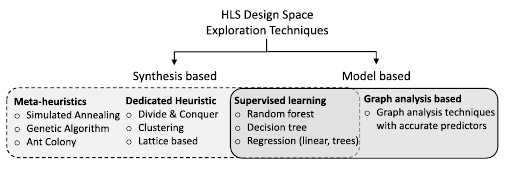
\includegraphics[width=1.0\textwidth]{Figures/HLS-taxonomy}
        \caption[Taxonomy for HLS based DSE approaches]{Taxonomy for HLS based DSE approaches, as proposed by Schafer \etal{} \cite{schafer_high-level_2020}}
        \label{ch.state:sec.strategies:fig.taxonomy}
    \end{figure}

    On the other hand, Barone \etal{} \cite{barone_multi-objective_2021} expose a substantial literature for \myAc{AxC}-based exploration, showing that specific domains have their own optimization problems, and claim that we need generic \myAc{DSE} framework to address those specificities.

    This section will thus expose a set of exploration initiatives based on introduced taxonomy from Schafer \etal{} \cite{schafer_high-level_2020} (Fig. \ref{ch.state:sec.strategies:fig.taxonomy}), and provide some insights about usage and limitations of considered approaches.

    \subsection{Meta Heuristics}
    \label{ch.state:sec.strategies:ssec.meta}
        A first class of exploration algorithms is based on meta heuristics, which are problem-independent heuristics that can be used to efficiently solve \myLongAcs{MOP}{Multi-objective Optimization Problem}.

        To begin with, \myLongAcs{GA}{Genetic Algorithm} have been used to perform \myAc{MOP} solving in an efficient way \cite{manuel_model-based_2020}.
        \myAc{GA} are evolutionary algorithms that relies on performing biologically inspired operations to evolve population toward better solutions, by model variations of implementation as potential mutations in a population of architecture.
        Dovado \cite{paletti_dovado_2021} exploit a {\bf Non-Dominated Genetic Algorithm} from \cite{shokri_algorithm_2013} to solve the \myAc{DSE} optimization problem, while Barone \etal{} \cite{barone_multi-objective_2021} provide an evolutionary search engine Bellerophon in their \eidea{} automatic exploration framework.
        This framework itself is an amelioration of $\mathbb{I}$DE$\mathbb{A}$ framework \cite{barbareschi_automatic_2016}, which was using a branch-and-bound approach to solve this optimization problem.

        We can also consider stochastic processes such as {\bf Bayesian optimization} for \myAc{MOP} solving, which can be used to optimize costly (\ie long to estimate) functions in an efficient fashion.
        To do so, multi-variate spaces are modelled using {\bf Gaussian processes} \cite{lo_model-based_2016}\cite{lo_multi-fidelity_2018}, and space exploration is then performed without having to exhaustively explore the whole space.
        This is the approach used by {\bf BOOM-Explorer} to efficiently propose a performant implementation of the \myAc{BOOM} core \cite{bai_boom-explorer_2021}: {\bf Gaussian processes} are used for initial set characterization (along with machine learning techniques), and {\bf Bayesian optimization} is then used for Pareto optimization of considered design space.

        Other meta heuristics for optimization have been exposed by Schafer \etal{} \cite{schafer_high-level_2020}, where biological and natural behaviours are used as model for optimization process, as it is the case with simulated annealing, for example.
        Simulated annealing is a Monte Carlo based method aiming to model the process of metal annealing, consisting in heating and cooling the metal in order to achieve a better stability.
        It can be used to approximate a global optimum for an optimization problem, by allowing to avoid local optima which could be found by simpler strategies, and was used to solve \myAc{DSE} problem by various initiatives, including Witschen \etal{} \cite{witschen_circa_2019}.

        As meta heuristic usage for \myAc{MOP} solving is a very wide research domain, we will not list every initiative to provide efficient manners of solving such problem.
        However, one should know that many algorithms can be used, and should consider them when building a \myAc{DSE} framework.        

    \subsection{Dedicated Heuristics}
    \label{ch.state:sec.strategies:ssec.dedicated}
        While meta-heuristics are problem-independent heuristics for optimization, dedicated heuristics are designed for specific problem solving.
        As \myAc{DSE} problem has been considered for decades now, many initiatives have proposed dedicated algorithms to perform efficient exploration, instead of trying to apply generic heuristics from other optimization domains.

        While Prost-Boucle \etal{} \cite{prost-boucle_fast_2014} propose a greedy approach to synthesize C algorithms under constraints (selecting and applying transforms in a sequential way to find Pareto optima), other approaches focus on quick estimation methodologies to perform exhaustive search of the space \cite{zhong_design_2017}\cite{bannwart_perina_fast_2021}.
        Other approaches uses the structure of design space itself to perform more efficient optimizations: for example, {\bf random sampling} of the space can be used, either to easily find Pareto optimum designs through neighbourhood exploration \cite{ye_scalehls_2021}, or to identify {\bf regions of interests} before performing sub region exploration through other processes such as search tree algorithms \cite{awais_ldax_2021}.
        In order to provide efficient exploration of the space, one can also consider iterative processes in a greedy approach --- \eg iteratively selecting next directive to optimize in \myAc{HLS} based processes \cite{siracusa_comprehensive_2021}, or using gradient based algorithms to find local optimum \cite{witschen_circa_2019}.

\clearpage
        Moreover, dedicated heuristics can also be defined for application specific explorations, with a rising needs for \myLongAc{CNN}{Convolutional Neural Network} implementation exploration \cite{motamedi_design_2016}\cite{park_roofline-model-based_2020}.
        This exhibits the specificities a domain can bring to the exploration problem, as well as the need for users to define specific explorations strategies for their use cases.

        More complex initiatives leverage multi-fidelity estimation: Dong Liu \etal{} \cite{dong_liu_efficient_2016} perform \myAc{HLS} based estimation of the whole space, then perform pruning before syntheses, using {\bf Rival Penalized Competitive Learning} to efficiently synthesize remaining implementations.
        In this way, they expose a need for a way to explicitly specify sequential exploration strategies to build complex strategy, while leveraging supervised learning methods to achieve efficient exploration.

    \subsection{Supervised Learning}
    \label{ch.state:sec.strategies:ssec.ml}
        As defined in exploration taxonomy from Figure \ref{ch.state:sec.strategies:fig.taxonomy}, both meta-heuristics and dedicated heuristics are synthesis based processes, meaning that they only consider synthesis (or other estimators) results to guide exploration.

        On the other hand, model based initiatives have been proposed in order to reduce the number of estimation processes to be run in an exploration process, thus accelerating the global flow.
        Supervised learning methods have thus emerged, leveraging synthesis generated knowledge to feed learning methods to be exploited later in the flow.

        Different uses of supervised learning have been proposed, from leveraging knowledge from prior explorations to speed-up the current one \cite{ferretti_leveraging_2020}, to fast simulated annealing using a decision tree \cite{mahapatra_machine-learning_2014}.
        
        Geng \etal{} \cite{geng_high-speed_2021} use {\bf Graph Neural Processing} to explore adder implementation, while Nardi \etal{} \cite{nardi_practical_2019} also leverage prior knowledge in {\bf Spatial} before using active learning under unknown feasibility constraints to provide Pareto approximation in their \myAc{DSE} engine.
        Liu \etal{} \cite{liu_learning-based_2013} study the usability of {\bf Random-Forest} algorithm for \myAc{HLS} based \myAc{DSE}, providing a comprehensive study on eight different learning models.
        Moreover, Meng \etal{} \cite{meng_adaptive_2016} provide an interesting approach to re-think machine learning usage for \myAc{DSE}, by using such methods to prune the design space before running end-to-end exploration using synthesis processes.

        Finally, {\bf BOOM-Explorer} \cite{bai_boom-explorer_2021} uses Gaussian process along with active learning and deep kernel learning functions for both initial set generation and design space characterization before employing Bayesian optimisation for exploration, showing that multiple approaches can be mixed to generate efficient exploration strategies.

    \subsection{Graph-Based Algorithms}
    \label{ch.state:sec.strategies:ssec.graph}
        The last class of \myAc{DSE} strategies in the considered taxonomy is purely based on modelling the whole synthesis flow instead of performing costly syntheses.

        Such initiatives include {\bf Lin-analyzer} \cite{zhong_lin-analyzer_2016}, which uses profiling to build a {\bf Dynamic Data Dependence Graph} (DDDG) model, {\bf COMBA} \cite{zhao_comba_2017}\cite{zhao_performance_2020}, a model based exploration framework for \myAc{HLS}, and {\bf FlexCL} \cite{wang_flexcl_2017}.
    
        This approach does expose the needs for expressivity for users to be able to build purely analytic models for exploration in their \myAc{DSE} framework.

    \subsection{Discussion on the Exploration Needs}
        A plethora of different approaches have been proposed in more or less recent initiatives in order to improve \myAc{DSE} processes, and various heuristics and algorithms should be considered by users aiming at implementing efficient exploration flows.

        Among those initiatives, some leverage multiple approaches by combining them for efficient exploration \cite{dong_liu_efficient_2016}\cite{bai_boom-explorer_2021}, displaying a need for flexibility in the process of building an exploration strategy ---  the designers should be able to define and guide their exploration based on both their applicative and technological expertises.

        In order to provide developers with such flexibility, a library of modular exploration passes should be proposed for efficient strategy building, allowing users to sequentially compose basic strategies to define more complex \myAc{DSE} operations in a given design space --- \eg leveraging quick estimation through learning methods for efficient pruning before running syntheses for more accurate results \cite{meng_adaptive_2016}.

\clearpage
\section{Synthesis on the Existing Approaches}
\label{ch.state:sec.synthesis}
    \subsubsection{Analysis of the literature}   
        In this chapter, we have provided an analysis of the existing \myLongAc{DSE}{Design Space Exploration} strategies in the literature, focussing on three main aspects --- the design space exposition, the metrics to be considered for both evaluation and comparison of different architectures, and the exploration strategies to be used to efficiently browse through a design space.

        We have identified some initiatives that could be considered to provide performant exploration frameworks, including wide research domains such as \myLongAc{HLS}{High Level Synthesis} and \myLongAcs{DSL}{Domain Specific Language}, and more recent approaches such as the \myLongAc{HCL}{Hardware Construction Language} paradigm.
        Among them, we put a particular focus on building flexible frameworks for strategy definition, such as the \myLongAc{AxC}{Approximate Computing} specific \eidea{} \cite{barone_multi-objective_2021}, which aims at proposing a generic exploration framework that allows its users to define application and target-independent strategies in an extensible fashion.

        In addition to this, we consider various taxonomies of exploration strategies, and among them the one proposed by Shathanaa \etal{} \cite{sa_design_2018}, where three strategy approaches are considered --- namely hierarchical approach, iterative approach, and sequential approach.
        We hereby identify an opportunity to leverage the composition of basic exploration strategies in a functional fashion, in order to provide the users with sequential approaches in their exploration framework.
    
    \subsubsection{Considered approach and planned contributions}
        Based on this analysis of the \myAc{DSE} research field, we plan to build an efficient exploration tool to ease the life of the hardware developers.
        More specifically, we examine providing a generic \myLongAc{FPGA}{Field-Programmable Gate Array} based exploration framework which would allow users to expose and control:
        \begin{itemize}
            \setlength\itemsep{-0.2cm}
            \item their own target and applicative domains
            \item their own design spaces
            \item their own metrics and estimation methodologies
            \item their own exploration strategies
        \end{itemize}
    
\clearpage
        To do so, the first step is hence to define how the design spaces are to be exposed in the framework.
        While we considered the usage of both \myAc{HLS} and \myAc{DSL}-based techniques for exposing explorable design spaces in this analysis, one can remark that such approaches have been widely explored in the past decades, resulting in the creation of multiple, industrially used frameworks.
        However, such tools are mainly based on the usage of architectural directives in the code to guide the exploration, and do not allow to finely control the generated accelerators as every choice that are not manually tuned by the developers are produced by automatic inference tools.
        On the other hand, some recent initiatives considered using \myLongAc{RTL}{Register-Transfer Level} languages to build generic exploration frameworks such as the one we are discussing here \cite{paletti_dovado_2021}.
        Nevertheless, they are based on standard \myLongAcs{HDL}{Hardware Description Language}, which are difficult to use and apprehend, and do not benefit from emerging paradigms to increase the productivity of the designers.
        To cope with those limitations, we hence consider using an \myAc{HCL} and its associated \myLongAc{HCF}{Hardware Construction Framework} to provide users with high level features for hardware development, while enabling to efficiently expose expertise-based design spaces.

        % As for the two other concerns --- namely the definition of the metrics of interests (as well as the corresponding estimation methodologies) and the description of the exploration strategies --- we consider implementing commonly used methodologies and algorithms as a {\it proof of concept}.
        As for the definition of the metrics of interest, as well as the corresponding estimation methodologies, we consider implementing the most commonly used methodologies as a {\it proof of concept}.
        However, some other approaches among the ones that have been presented in this chapter could be applied to build meaningful ways to evaluate and compare architectures, in order to provide users with both modularity and flexibility in their design processes.
        Indeed, some other initiatives cannot be applied in this context --- \eg considering an \myAc{HCL} as the entry point of the exploration flows is not compatible with the estimation methodologies that rely on an algorithmic description of the circuits behaviours, as it is the case for most of the \myAc{HLS}-based latency and resource estimators.

        Finally, when it comes to the exploration strategies, most of the considered algorithms can be applied for \myAc{DSE} regardless of the exposition of the design space --- except for graph-based algorithms, which also require an algorithmic description to be used.
        In this context, and even if we only consider implementing basic strategies in a first time, one could consider each of those approaches to build a configurable library of exploration algorithms, hence providing the users with a generic and modular tool.

\clearpage
    \subsubsection{Identified limitations}

        After defining the scope of this work, as well as the planned contributions, we identify some limitations about the proposed approach.

        First of all, it will require its users to explicitly expose the design space, thus requiring expertise about both the algorithm and the target board.
        It is quite different from the \myAc{HLS} approach, for example, where the design space is essentially defined by the transformations performed by the \myAc{HLS} tool to generate the accelerators, that are quite transparent for the developers.

        Moreover, our approach will require the users not only to define the design space to be explored (by exposing the generation parameters as architectural knobs), but also to describe the different generators of accelerators in a \myAc{RTL}-based language, which also requires a lot of time and expertise.

        Last but not least, we will only consider sequential exploration strategies in this work, which could be a limitation for the algorithms relying on parallel and interacting steps for instance.
        
        However, we propose to explore the opportunity of building a fully configurable exploration framework, that would leverage the features of recent \myAcs{HCF} to facilitate the life of hardware developers.


%%%%%%%%%%%%%%%%%%%%%%%%%%%%%%%%%%%%%%%%%%%%%%%%%%%%%%%%%%%%%%%%%%%%%%%%%%%%%%%%
%%%%%%%%%%%%%%%%%%%%%%%%%%%%%%%%%%%%%%%%%%%%%%%%%%%%%%%%%%%%%%%%%%%%%%%%%%%%%%%%
